%% LaTeX Beamer presentation template (requires beamer package)
%% see http://bitbucket.org/rivanvx/beamer/wiki/Home
%% idea contributed by H. Turgut Uyar
%% template based on a template by Till Tantau
%% this template is still evolving - it might differ in future releases!


\documentclass{beamer}
 
\mode<presentation>
{
\usetheme{NYU}

\setbeamercovered{transparent}
}

\usepackage[english]{babel}
\usepackage[latin1]{inputenc}

% font definitions, try \usepackage{ae} instead of the following
% three lines if you don't like this look
\usepackage{mathptmx}
\usepackage[scaled=.90]{helvet}
\usepackage{courier}


\usepackage[T1]{fontenc}


\usepackage{comment}
%usepackage{appendixnumberbeamer}
%\usepackage{amsmath}
\usepackage{pgfpages}
\usepackage{float}
% citations
\usepackage{natbib}
\usepackage{lipsum}
\usepackage[export]{adjustbox}
\usepackage{subfig}

\bibpunct{(}{)}{;}{a}{,}{,}
\def\citeapos#1{\citeauthor{#1}'s (\citeyear{#1})}
\renewcommand{\bibsection}{\subsubsection*{\bibname } }

\title{Predicting FOMC Actions Using ML and NLP}

%\subtitle{}

% - Use the \inst{?} command only if the authors have different
%   affiliation.
%\author{F.~Author\inst{1} \and S.~Another\inst{2}}
\author{Jeremy Lao - jjl359  \& John Reynolds - jr4716} 

% - Use the \inst command only if there are several affiliations.
% - Keep it simple, no one is interested in your street address.
\institute[NYU]
{
Department of Computer Science\\
Courant Institute of Mathematical Sciences, NYU\\
  \texttt{}
}

\date{May-7-2019}


% This is only inserted into the PDF information catalog. Can be left
% out.
\subject{Subject}



% If you have a file called "university-logo-filename.xxx", where xxx
% is a graphic format that can be processed by latex or pdflatex,
% resp., then you can add a logo as follows:

\pgfdeclareimage[height=0.5cm]{university-logo}{nyu_long_color}
\logo{\pgfuseimage{university-logo}}




% If you wish to uncover everything in a step-wise fashion, uncomment
% the following command:

%\beamerdefaultoverlayspecification{<+->}

\begin{document}




\begin{frame}
\frametitle {Predicting FOMC Actions Using ML and NLP  \\Jeremy Lao - jjl359  \& John Reynolds - jr4716 }

\small \textbf{Model-1: FOMC Decison $D_t$ based on lagged document text}
\vspace{-2mm}
\begin{small}
$$E[D_t | \mbox{Statements}_{t-i}, \mbox{Minutes}_{t-j} , \mbox{Speeches}_{t-k}, \mbox{N-gram}]$$
\end{small}
\vspace{-2.5mm}
\small \textbf{Model-2: FOMC Decison $D_t$ based on aggregated lagged document text}
\begin{small}
$$E[D_t | \mbox{AGG}(\mbox{Statements}_{t-i}, \mbox{Minutes}_{t-j} , \mbox{Speeches}_{t-k}), \mbox{N-gram}]$$
\end{small}

\vspace{-7mm}

\noindent \center {\small where} {$D_t = 1$}{\small, if change to rates,} {$D_t = 0$}{\small, if no change.}


\vspace{-5mm}
\begin{figure}[h]
  \subfloat
   {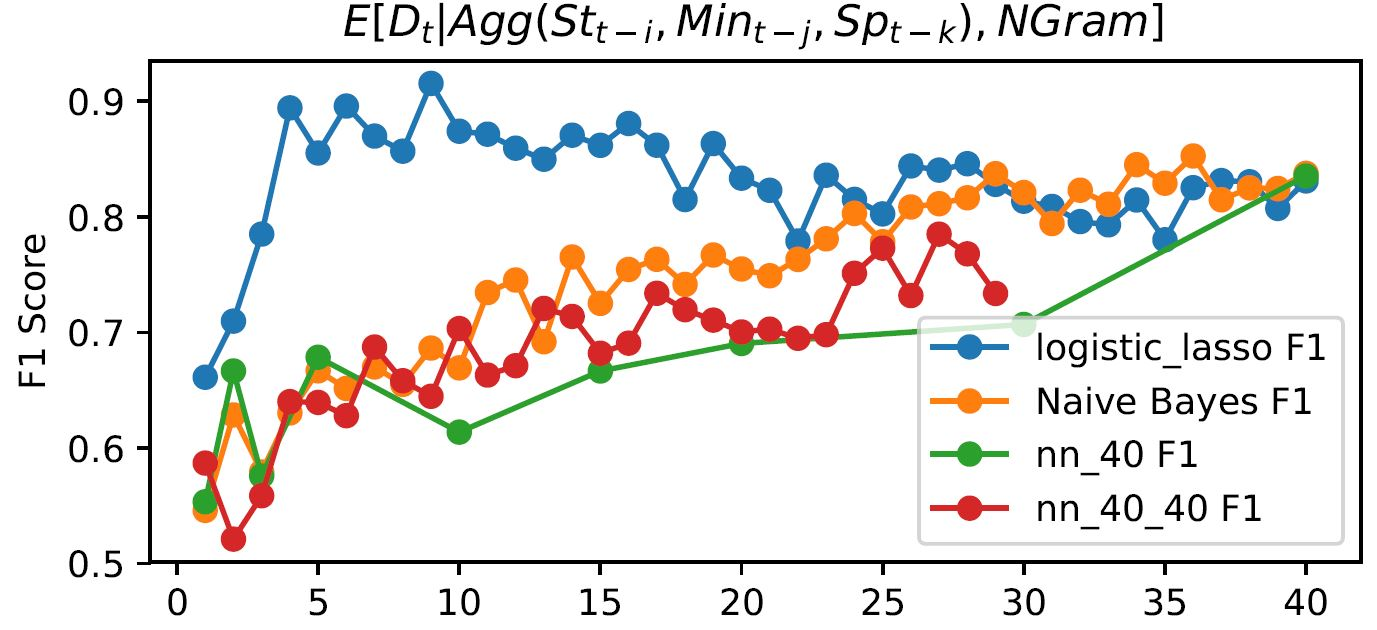
\includegraphics[width=.5\textwidth]{./model1.jpg}  
   \hspace{10px}} 
  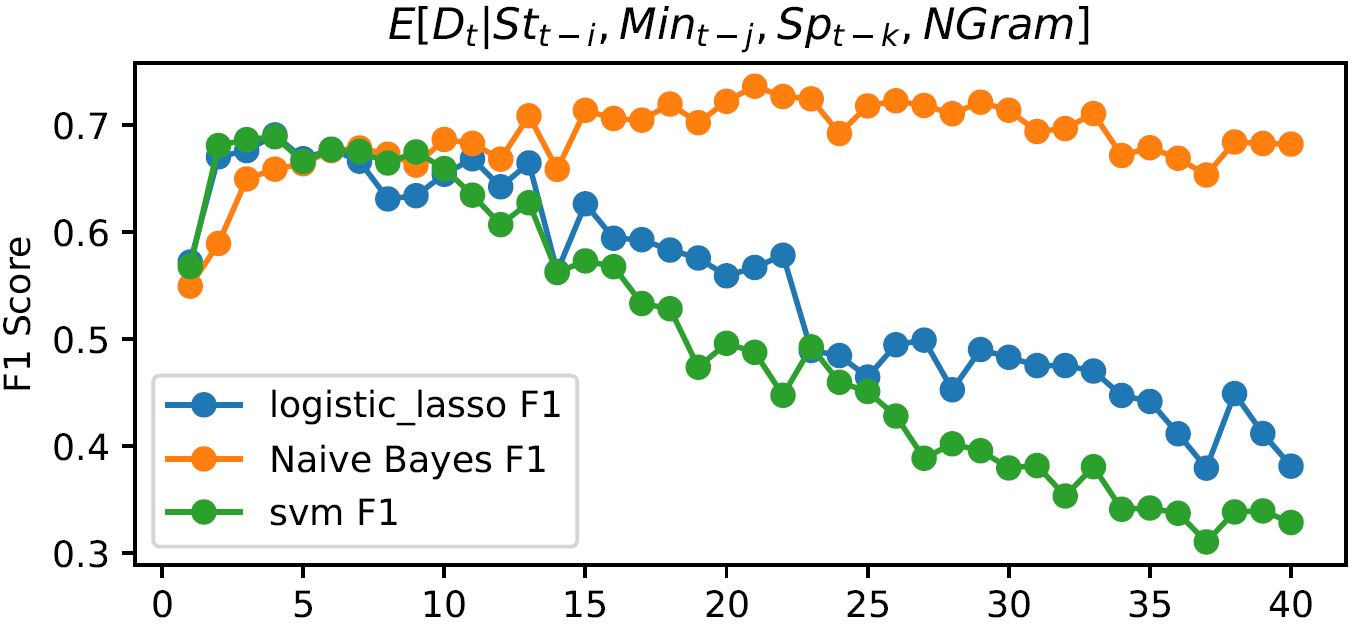
\includegraphics[width=.5\textwidth]{./model2.jpg}
  \captionsetup{labelformat=empty}
  \caption{x-axis: Ngram, y-axis: F1 Score}
\end{figure}



\end{frame}


\end{document}
